\documentclass{beamer}
\mode<presentation>
{
  \usetheme{Montpellier}
  \usefonttheme{structuresmallcapsserif}
  \setbeamercovered{transparent}
}

\usepackage[backend=biber]{biblatex}
\usepackage[english]{babel}
\usepackage[utf8]{inputenc}

\usepackage{helvet}

\usepackage{hyperref} 

\hypersetup{
    colorlinks=true,   
    linkcolor=blue,    
    filecolor=magenta, 
    urlcolor=cyan,     
    bookmarks=true,      
    bookmarksopen=true,  
}


\usepackage{tikz}
\usepackage{amscd, amssymb, amsmath, amsthm}
\usepackage{bbm}
\usepackage{amsfonts,amssymb}
\usepackage{epsfig,epstopdf}
\usepackage{url,array}
%\usepackage{titling}
\usetikzlibrary{decorations.markings,calc}
\usepackage{amsthm}
\usepackage{subfig}


\usepackage[all]{xy}
\usetikzlibrary{hobby}    
%%%%%%%%%%%%%%%%%%%


\usefonttheme{serif}
\setbeamerfont{structure}{family=\rmfamily}


\pdfsuppresswarningpagegroup=1

\newtheorem{thm}{Theorem}[section]
\newtheorem{lem}[thm]{Lemma}
\newtheorem{prop}[thm]{Proposition}
\newtheorem{cor}[thm]{Corollary}
\newtheorem{proposition}[theorem]{Proposition}

\theoremstyle{definition}
\newtheorem{df}[thm]{Definition}
\newtheorem{conj}{Conjecture}[section]
\newtheorem{exmp}{Example}[section]

\theoremstyle{remark}
\newtheorem*{rem}{Remark}



%Inequalities
\newcommand{\cycsum}{\sum_{\mathrm{cyc}}}
\newcommand{\symsum}{\sum_{\mathrm{sym}}}
\newcommand{\cycprod}{\prod_{\mathrm{cyc}}}
\newcommand{\symprod}{\prod_{\mathrm{sym}}}

%Linear Algebra

\DeclareMathOperator{\Span}{span}
\DeclareMathOperator{\Ima}{Im}
\DeclareMathOperator{\diag}{diag}
\DeclareMathOperator{\Ker}{Ker}
\DeclareMathOperator{\ob}{ob}
\DeclareMathOperator{\Hom}{Hom}
\DeclareMathOperator{\sk}{sk}
\DeclareMathOperator{\Vect}{Vect}
\DeclareMathOperator{\Set}{Set}
\DeclareMathOperator{\Group}{Group}
\DeclareMathOperator{\Ring}{Ring}
\DeclareMathOperator{\Ab}{Ab}
\DeclareMathOperator{\Top}{Top}
\DeclareMathOperator{\hTop}{hTop}
\DeclareMathOperator{\Htpy}{Htpy}
\DeclareMathOperator{\Cat}{Cat}
\DeclareMathOperator{\CAT}{CAT}
\DeclareMathOperator{\Cone}{Cone}
\DeclareMathOperator{\dom}{dom}
\DeclareMathOperator{\cod}{cod}
\DeclareMathOperator{\Aut}{Aut}
\DeclareMathOperator{\Mat}{Mat}
\DeclareMathOperator{\Fin}{Fin}
\DeclareMathOperator{\rel}{rel}
\DeclareMathOperator{\Int}{Int}
\DeclareMathOperator{\sgn}{sgn}
\DeclareMathOperator{\PSL}{PSL}
\DeclareMathOperator{\Supp}{Supp}
\DeclareMathOperator{\tr}{tr}

%Row operations
\newcommand{\elem}[1]{% elementary operations
\xrightarrow{\substack{#1}}%
}

\newcommand{\lelem}[1]{% elementary operations (left alignment)
\xrightarrow{\begin{subarray}{l}#1\end{subarray}}%
}

%SS
\DeclareMathOperator{\supp}{supp}
\DeclareMathOperator{\Var}{Var}

%NT
\DeclareMathOperator{\ord}{ord}

%Alg
\DeclareMathOperator{\Rad}{Rad}
\DeclareMathOperator{\Jac}{Jac}

%Misc
\newcommand{\SL}{{\mathrm{SL}}}
\newcommand{\mobgp}{{\mathrm{PSL}_2(\mathbb{C})}}
\newcommand{\id}{{\mathrm{id}}}
\newcommand{\Mod}{{\mathrm{Mod}}}
\newcommand{\SMod}{{\mathrm{SMod}}}
\newcommand{\PMod}{{\mathrm{PMod}}}
\newcommand{\ud}{{\mathrm{d}}}
\newcommand{\Vol}{{\mathrm{Vol}}}
\newcommand{\Area}{{\mathrm{Area}}}
\newcommand{\diam}{{\mathrm{diam}}}
\newcommand{\Homeo}{{\mathrm{Homeo}}}
\newcommand{\SHomeo}{{\mathrm{SHomeo}}}


\newcommand{\reg}{{\mathtt{reg}}}
\newcommand{\geo}{{\mathtt{geo}}}

\newcommand{\tori}{{\mathcal{T}}}
\newcommand{\cpn}{{\mathtt{c}}}
\newcommand{\pat}{{\mathtt{p}}}

\let\Cap\undefined
\newcommand{\Cap}{{\mathcal{C}}ap}
\newcommand{\Push}{{\mathcal{P}}ush}
\newcommand{\Forget}{{\mathcal{F}}orget}




\title[Mapping Class Groups, Braid Groups and Geometric Representations] {Riemann surfaces underlying 
$K_n$-dessins}

\author{Jonas Trepiakas}



\date{} 

\subject{Talks}

\AtBeginSubsection[]
{
  \begin{frame}<beamer>{}
    \tableofcontents[currentsection,currentsubsection]
  \end{frame}
}


% If you wish to uncover everything in a step-wise fashion, uncomment
% the following command: 
%\beamerdefaultoverlayspecification{<+->}

\begin{document}



\section{Mapping Class Groups}

\begin{frame}{Definition}
    \begin{df}
        Let $S$ be a surface and
        $\Homeo^+ (S, \partial S)$
        denote the group of 
        orientation-preserving 
        self-homeomorphisms of $S$
        which fix the boundary
        pointwise.

        Equipping $\Homeo^+ 
    (S, \partial S)$ with the
    compact-open topology inherited
    from $C^0 (S,S)$, we
    define
    \[\Mod (S) :=
    \pi_0 (\Homeo^+ (S, \partial S)).\]
    \end{df}
\end{frame}

%\begin{frame}{Interpretation}
%    \begin{lem}
%        Let $X,Y,Z$ be Hausdorff spaces
%        with $Y$ locally compact. Then
%        a map $f \colon 
%        X \to C_W^0 (Y,Z)$ is
%        continuous if and only if
%        $F \colon X \times Y \to 
%        Z$ defined by 
%        $F(x,y) = f(x)(y)$ is
%        continuous.
%    \end{lem}
%    Thus, a path
%    $\gamma \colon I \to \Homeo^+ 
%    (S, \partial S)$
%    is the same as
%    a continuous map
%    $I \times S \to S$ given by
%    $(t,s) \mapsto \gamma(t) (s)$
%    which is an isotopy of
%    $S$.
%\end{frame}


\section{Dehn Twists}

\begin{frame}{Definition of a Dehn Twist}

\begin{df}
    Define the left twist map
    of the annulus $A = S^1 \times
    [1,2]$ as
    $T \colon A \to A$ given by
    $T(\theta, t) = 
    (\theta + 2 \pi t, t)$.
\end{df}

    \begin{figure}
        \centering 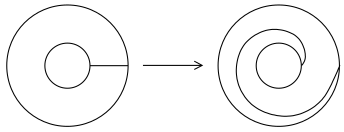
\includegraphics[width=0.4\linewidth]{dehn-twist-annulus.png}
        \label{fig:enter-label}
    \end{figure}    
    \begin{df}
        For an oriented surface $S$
        with a simple loop $\alpha$
        in $S$, let
        $N$ be a tubular neighborhood
        of $\alpha$ and choose
        an orientation-preserving
        homeomorphism 
        $\varphi \colon A \to N$.
        We define a \textit{Dehn twist about $\alpha$} as
        \[T_{\alpha} (x)
        = 
        \begin{cases}
            \varphi \circ T \circ
            \varphi^{-1}& x \in N\\
            x& x \in S - N
        \end{cases}
        \]
    \end{df}
\end{frame}

\begin{frame}{Braid Group Relations}
    \begin{prop}
        If $a,b$ are isotopy classes
        of simple closed curves, then
        $i(a,b) = 0$ if and only if
        $T_a T_b = T_b T_a$. 
        Furthermore, if
        $i (a,b) = 1$, then
        \[T_a T_b T_a = 
        T_b T_a T_b\].
    \end{prop}

\begin{df}
    The braid group on
    $n$ strands, $\mathcal{B}_n$, is
    the group generated by $\sigma_1,
    \ldots, \sigma_{n-1}$
    with the relations $\sigma_i \sigma_j = \sigma_j \sigma_i$ for
    $|i-j| > 1$ and 
    $\sigma_i \sigma_{i+1} \sigma_i 
    = \sigma_{i+1} \sigma_i \sigma_{i+1}$
    for all $i$.
\end{df}
\end{frame}

\begin{frame}{Geometric Representations}
    \begin{df}
        A geometric representation of a group $G$ is a homomorphism
        $G \to \Mod(S)$ where $S$ is a surface.
    \end{df}

    By the previous proposition on relations of Dehn-twists, we
    find that
    if we have a sequence of curves
    $\alpha_1, \ldots, \alpha_{n-1}$
    such that $i (\alpha_i, \alpha_{i+1})
    = 1$ for all $i$ and
    $i (\alpha_i, \alpha_j) = 0$ whenever
    $|i-j| > 1$, then
    we obtain a well-defined homomorphism
    $\mathcal{B}_n \to \Mod(S)$ by sending
    $\sigma_i \mapsto T_{\alpha_i}$.\\

    A collection of curves satisfying
    these conditions is called
    a chain of curves.
\end{frame}

\section{Yang-Baxter Operators}

\begin{frame}{Yang-Baxter Operators}

\begin{df}
    Let $T \colon
    \mathbbm{1} \to \mathcal{V}$
    be a functor into
    a monoidal category $\mathcal{V}$.
    A Yang-Baxter operator
    on $X:=T(*)$ is an automorphism
    \[y \in \Aut_{\mathcal{V}}(X \otimes X)\]
    such that the following diagram commutes
    \begin{figure}
        \centering
        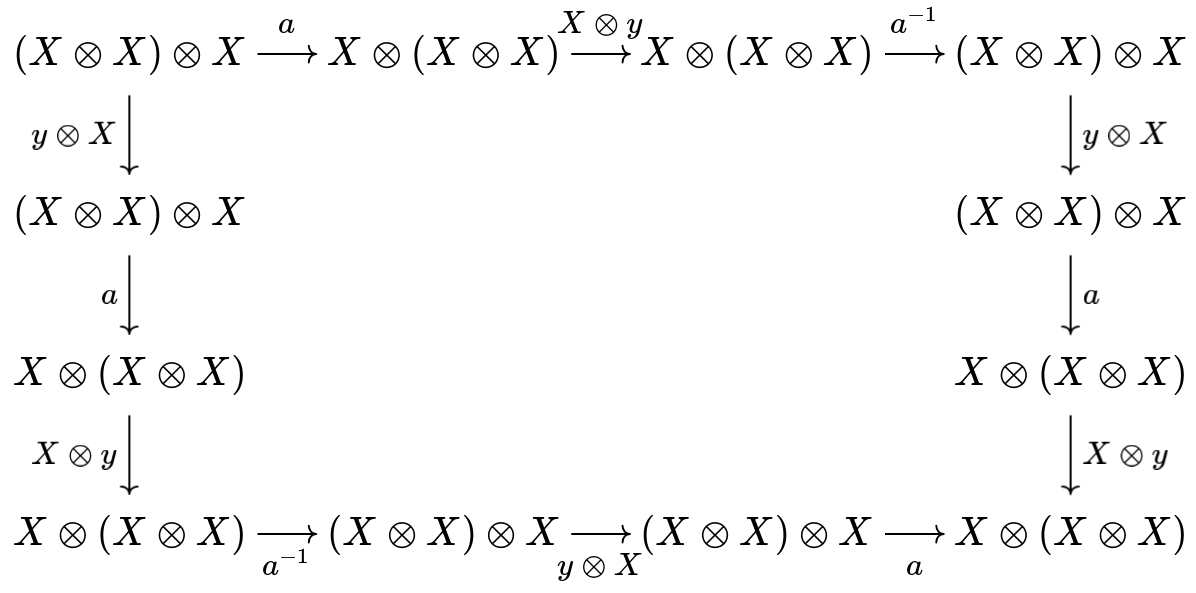
\includegraphics[width=0.6\linewidth]{Yang-Baxter-2.png}
        \label{fig:enter-label}
    \end{figure}
\end{df}
\end{frame}

\begin{frame}{Yang-Baxter operators}

If $T \colon  \mathbbm{1} \to
\mathcal{V}$ is a functor with
$\mathcal{V}$ braided monoidal, 
we obtain the Yang-Baxter operator
\[y = 
b_{X , X} \colon 
X \otimes X \stackrel{\sim}{\to} 
X \otimes X\]

We denote by
$z$ the Yang-Baxter operator
obtained in this way
from the inclusion functor
$\iota \colon \mathbbm{1} \to
\mathcal{B}$, where
$\mathcal{B}$ is the braid groupoid
and the inclusion maps
$\id$ to the single strand.
\end{frame}

\begin{frame}{Obtaining representations from Yang-Baxter operators}
    \begin{prop}
        For any strict monoidal category
        $\mathcal{V}$ and
        any Yang-Baxter operator
        $\tau$ on an element
        $X \in \mathcal{V}$, there
        exists a unique strict 
        monoidal functor 
        $\Phi_{X, \tau} \colon
        \mathcal{B} \to 
        \mathcal{V}$ such that
        $\Phi_{X, \tau} \circ z = y$.
    \end{prop}

    \begin{proof}
        Since $\Phi_{X,\tau}$ is strict
        monoidal, this forces
        $\Phi_{X,\tau} (A) \otimes
        \Phi_{X,\tau} (B) =
        \Phi_{X,\tau}(A \otimes B)$ which
        forces $\Phi_{X,\tau} 
        (n) = X^{\otimes n}$ and
        since $\sigma_i = 
        1 \otimes \ldots \otimes 1 \otimes
        \sigma_1 \otimes 1 \otimes \ldots
        \otimes 1$, it forces
        $\Phi_{X,\tau}(\sigma_i)
        = X \otimes \ldots \otimes
        X \otimes y \otimes X
        \otimes \ldots \otimes X =: y_i$.
        As $y$ is a Yang-Baxter operator
        and $\mathcal{V}$ is strict,
        these satisfy the braid group
        relations.
    \end{proof}
\end{frame}

\section{Categories of surfaces}

\begin{frame}{Braided monoidal category of decorated surfaces}

The definition and figures for this section were taken from a paper by Nathalie Wahl and Oscar Randal-Williams

    \begin{df}
        A decorated surface is a pair
        $(S, I)$ where $S$ is a 
        compact connected surface 
        with at least one boundary
        component, and
        $I \colon [-1,1] 
        \hookrightarrow \partial S$
        is an interval in the boundary.

        Let $\mathcal{M}_1$ be
        the groupoid where the objects
        are decorated surfaces and
        morphisms are isotopy classes of
        homeomorphisms restricting to
        the identity on a neighborhood
        of $I$ and fixing the other boundaries. 
    \end{df}

    Then $\Aut_{\mathcal{M}_1}(S)
    = \Mod(S)$.
\end{frame}

\begin{frame}{The Monoidal Structure}
     We equip it with the
     monoidal structure 
     $(S_1, I_1) \otimes
     (S_2, I_2) :=
     (S_1 \natural S_2, I_1 \natural
     I_2)$ where
     $I_1 \natural I_2 = I_1^{-}
     \cup I_2^{+}$ and
     $S_1 \natural S_2$ is obtained
     by gluing $S_1$ and
     $S_2$ along $I_1^+$ and
     $I_2^-$
     \begin{figure}
         \centering
         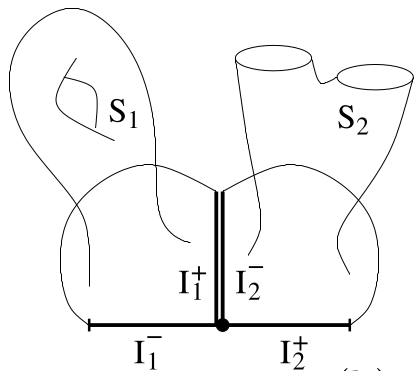
\includegraphics[width=0.3\linewidth]{connected-sum.png}
         \label{fig:enter-label}
     \end{figure}

\end{frame}

\begin{frame}{The Braiding}
The braiding is defined by a half twist
of a pair-of-pants neighborhood of
$\partial S_1 \cup \partial S_2$
    \begin{figure}
        \centering
        \includegraphics[width=0.25\linewidth]{braidingM2.png}
        \label{fig:enter-label}
    \end{figure}

    By the proposition, we
    obtain a monoidal functor
    $\Phi \colon \mathcal{B} \to
    \mathcal{M}_1$ such that
    $\Phi \circ z = y$ where
    $y$ is the Yang-Baxter operator on
    some decorated surface
    $S$ which corresponds to
    the half-Dehn twist.
\end{frame}

\section{Geometric Representations
of the Braid Group}

\begin{frame}{The main goal}
    Recall that 
a geometric representation of a group
$G$ is a group homomorphism
$G \to \Mod(S)$ for some surface $S$.

The following theorem was proved by Stukow and Szepietowski, and the figures for the representations were taken from their paper

\begin{thm}
    Let $n \geq 14$ and
    $N = N_{g,b}$ with $g \leq 
    2 \lfloor \frac{n}{2} \rfloor + 1
    $ and $b \geq 0$. Then any 
    geometric representation 
    $\mathcal{B}_n \to \Mod(N)$
    is, up to transvection, either trivial, a standard twist representation or a crosscap transposition representation.
\end{thm}

The goal is to find out
whether these representations
can be obtained from Yang-Baxter operators
on an appropriately chosen
category of surfaces.
\end{frame}

\begin{frame}{The crosscap transposition representation}

Given the setup in the figure with
$\mu_i$ the core
curve of the Möbius band
$K_i - K_{i-1}$, we
let $u_i$ be the crosscap transposition
supported in $K_i$ which
swaps $\mu_i$ and $\mu_{i+1}$ and
$u_i^2 = T_{a_i}$ - i.e., a
half-twist of the crosscaps.

    \begin{figure}
        \centering
        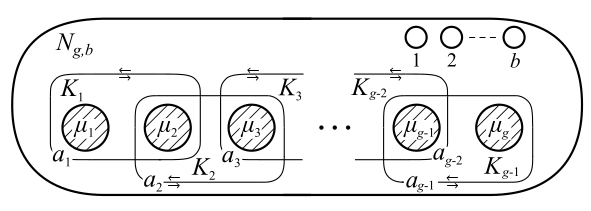
\includegraphics[width=0.6\linewidth]{chain-separating-curves.png}
        \label{fig:enter-label}
    \end{figure}

The mapping $\theta_C \colon
\mathcal{B}_n \to 
\PMod(N)$ sending $\sigma_i \mapsto
u_i$ is called the crosscap transposition representation.

It is clear that this is the representation induced by the braiding from $\mathcal{M}_1$ (the half-twist on a pairs-of-pants neighborhood) on the Möbius band.
\end{frame}

\begin{frame}{The standard twist representation}

Take a chain of two-sided curves
$C = (a_1, \ldots , a_{g-1})$ as
depicted in the figure and fix
an orientation of a regular neighborhood
of their union.
Then the map
$\rho_C \colon \mathcal{B}_n 
\to \PMod(S)$ defined by
$\rho_C (\sigma_i) = T_{a_i}$
is called the standard twist representation.

\begin{figure}
    \centering
    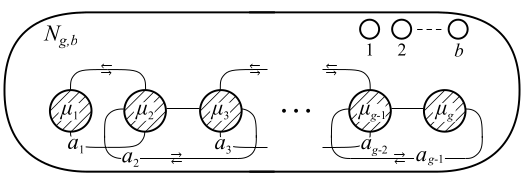
\includegraphics[width=0.7\linewidth]{standard-chain.png}
    \label{fig:enter-label}
\end{figure}
    
\end{frame}


\begin{frame}{The Yang-Baxter Operator}

We can obtain the standard twist representation as the Yang-Baxter element on the Möbius band $M$ given by
a Dehn twist about the
curve denoted in the figure
below for $M \natural M$.

\begin{figure}[H]
    \centering
    \begin{minipage}[b]{0.5\textwidth}
        \centering
        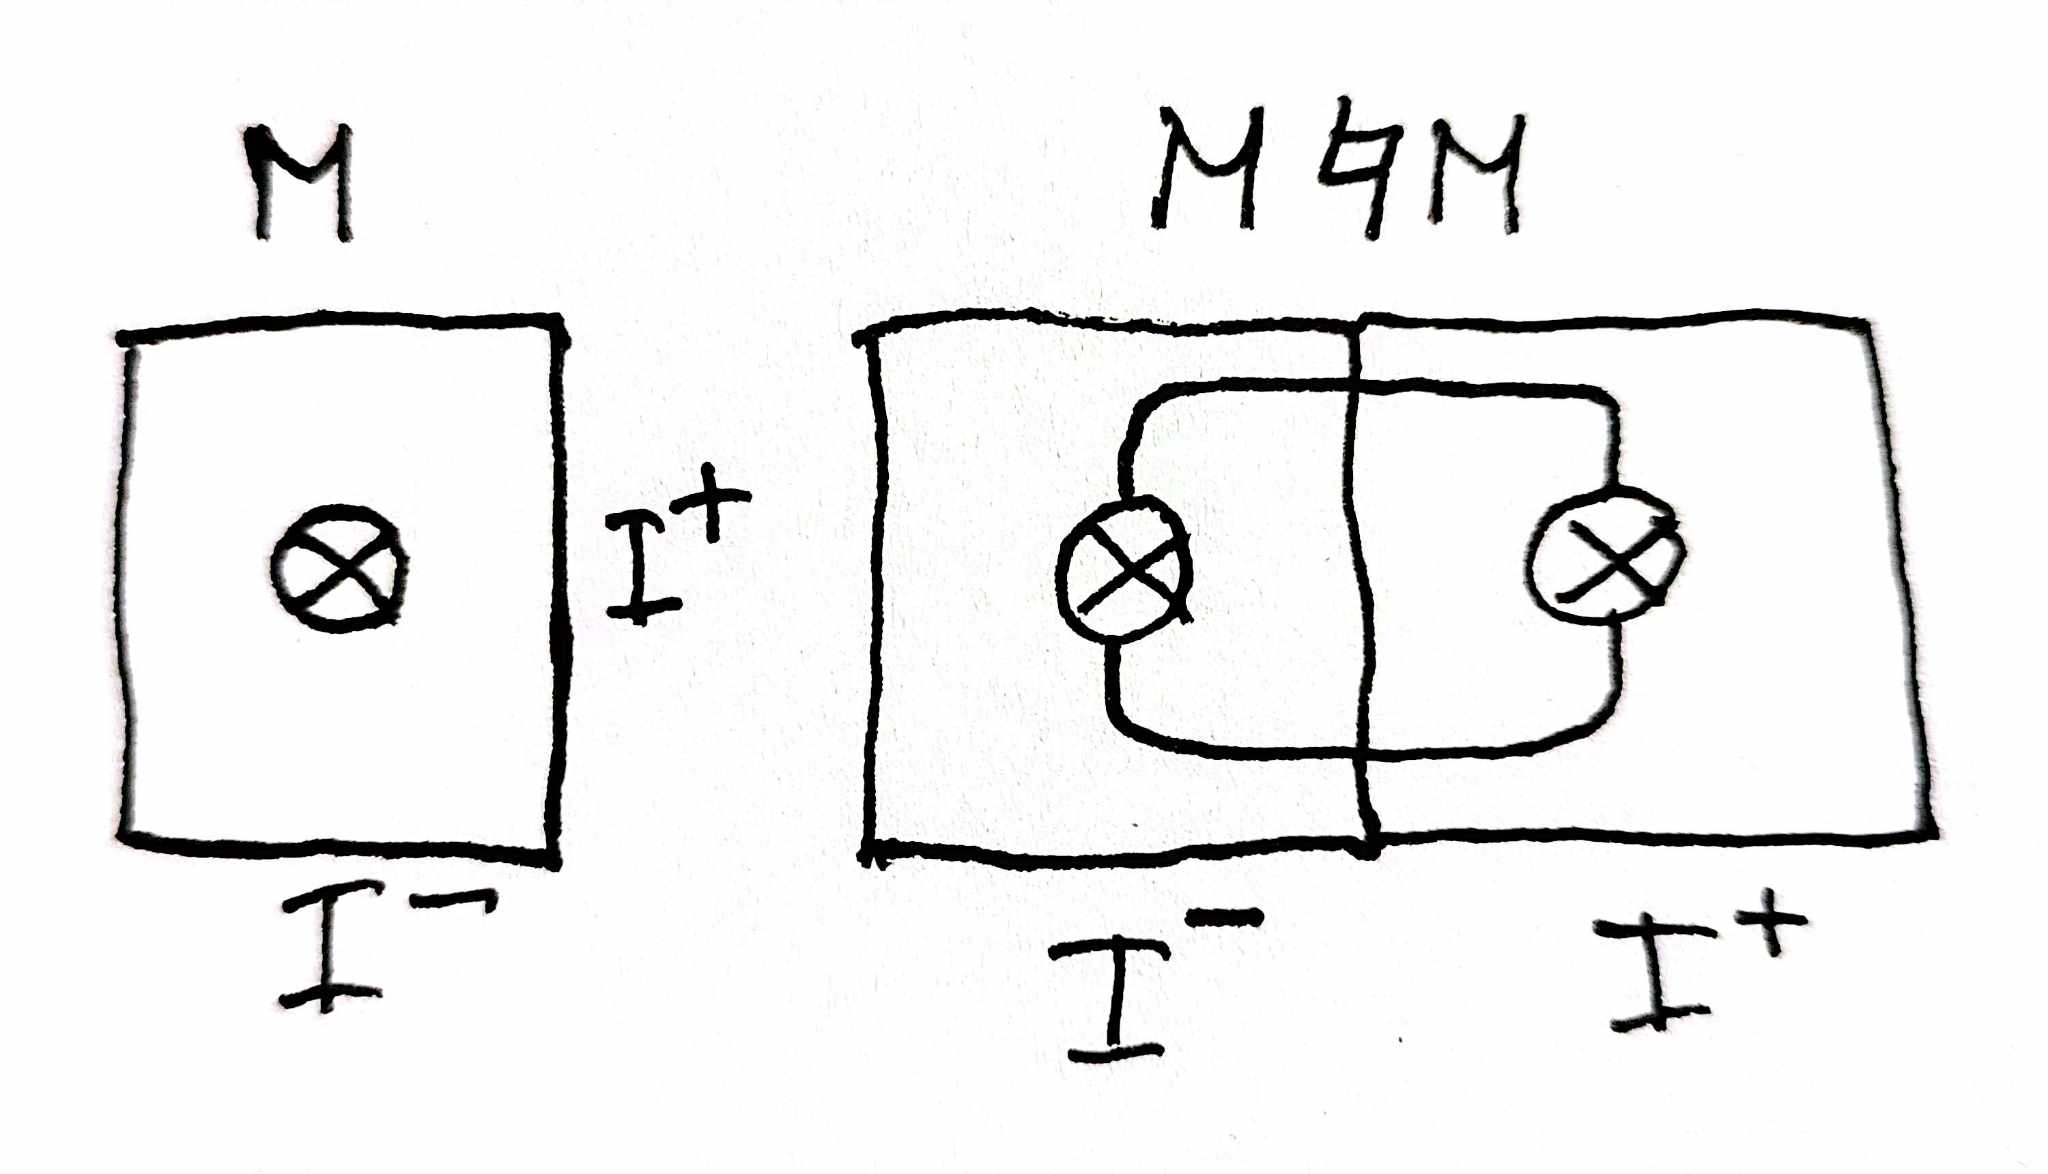
\includegraphics[width=0.8\textwidth]{mobius-decorated.jpg} % first figure itself
    \end{minipage}\hfill
    \begin{minipage}[b]{0.5\textwidth}
        \centering
        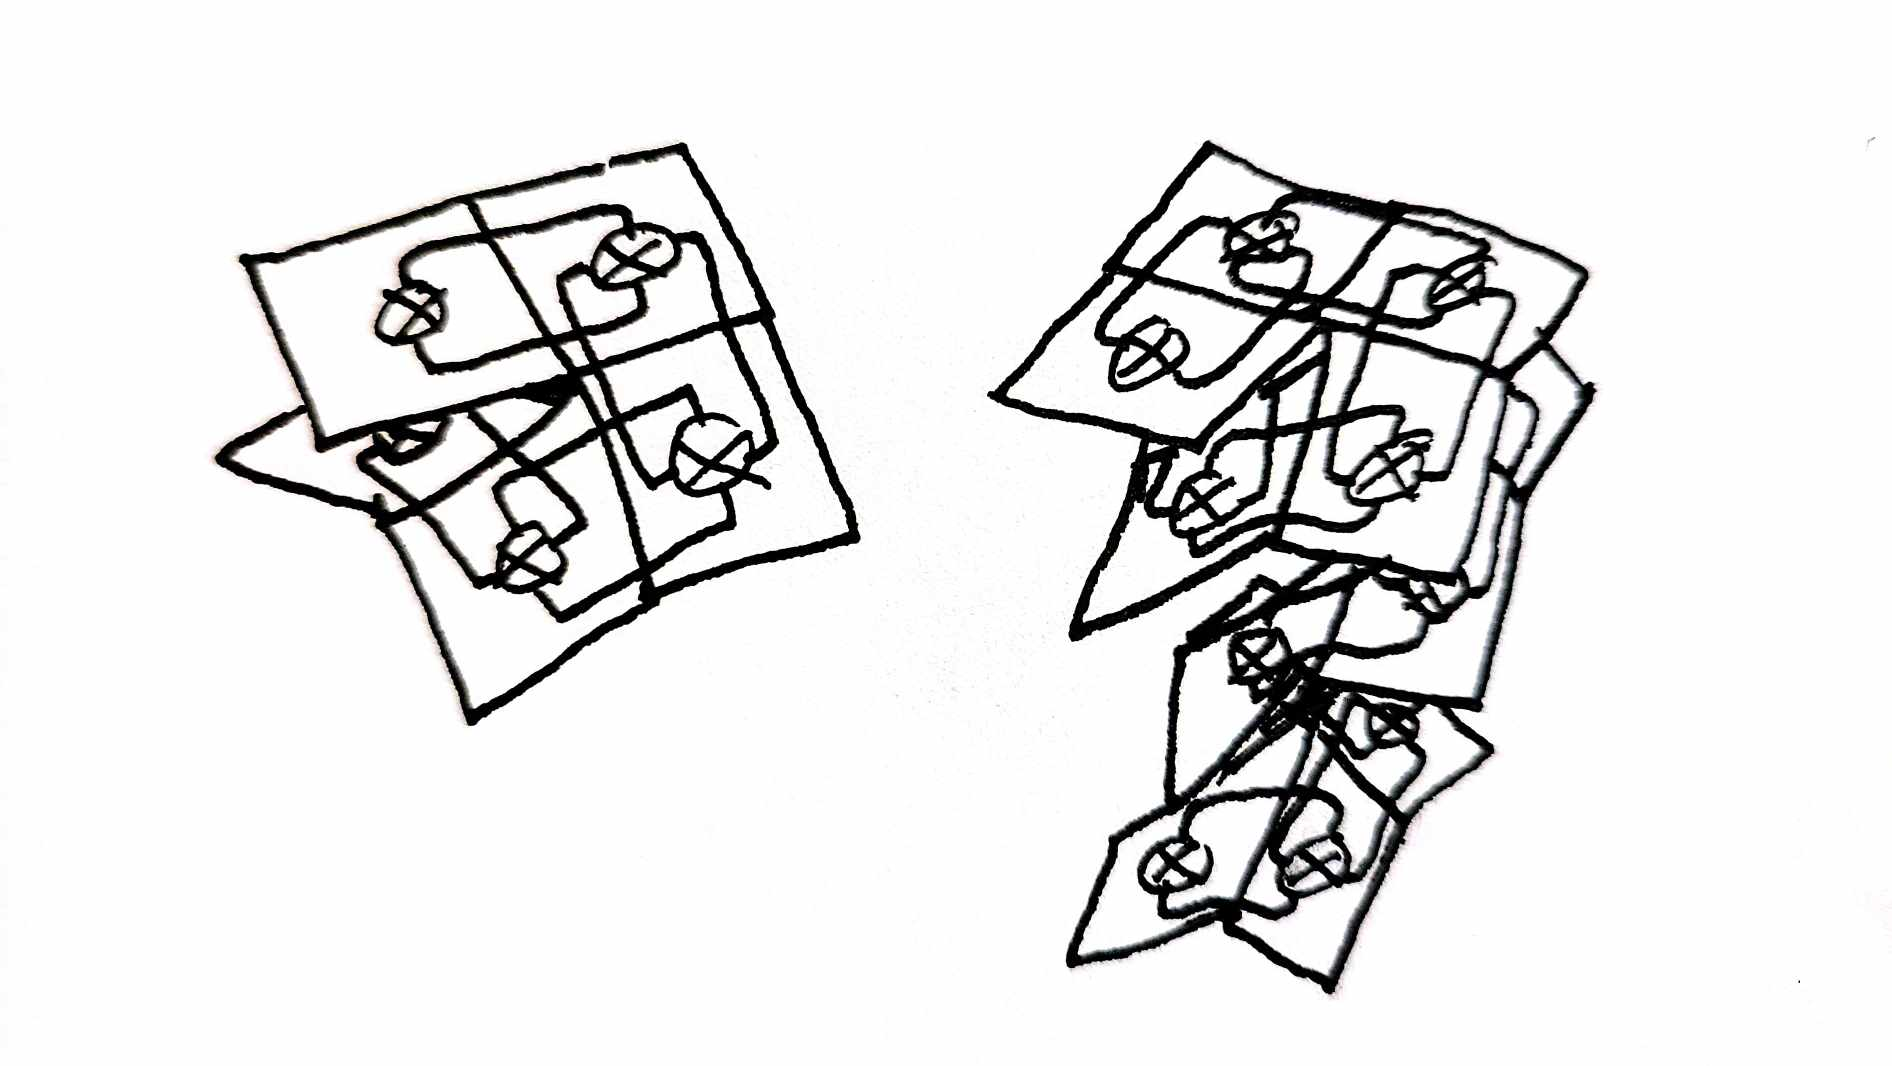
\includegraphics[width=1.2\textwidth]{Ng1.jpg} % second figure itself
    \end{minipage}
\end{figure}
\end{frame}

\begin{frame}{Recovering the
Birman-Hilden embedding}
    \begin{prop}
        For $b\geq 1$ and $g$ odd,
        the standard twist representation
        $\rho_C \colon \mathcal{B}_g
        \to \Mod(N_{g,b})$ is the
        same as the Birman-Hilden embedding $B_g \hookrightarrow
        S_{\frac{g-1}{2},b-1} 
        \# M$ into the orientable
        factor.
    \end{prop}
\end{frame}

\begin{frame}{Proof}
    We first note that
    $T^2 \# M \approx
    K \# M$



    \begin{figure}
        \centering
        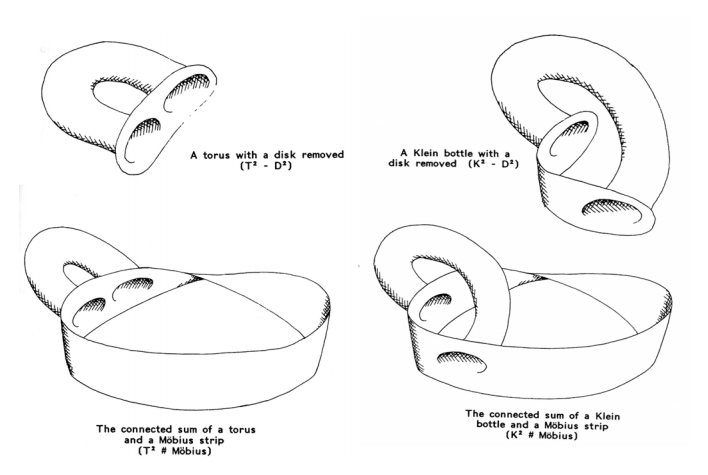
\includegraphics[width=0.75\linewidth]{N_3,1.jpg}
        \caption{This figure was taken from the book "The shape of space" by Jeffrey R. Weeks}
        \label{fig:enter-label}
    \end{figure}
\end{frame}

\begin{frame}{Proof}
We will follow the loops through
the following chain of
homeomorphisms
    \begin{align*}
N_{2n+1,1} \approx
\left( \mathbb{R}\mathbb{P}^2 \right)^{\# 2n+1} -
\mathring{D} 
&\approx K^{\# n} \# M
\approx K^{\# n-1} \# K \# M\\
&\approx K^{\# n-1} \# T^2 \# M\\
&\vdots\\
&\approx \left( T^2 \right)^{\# n} \# M\\
&\approx S_{n,0} \# M\\
&\approx S_{n,1} \natural M
\end{align*}
\end{frame}

\begin{frame}{Proof}
    \begin{figure}
        \centering
        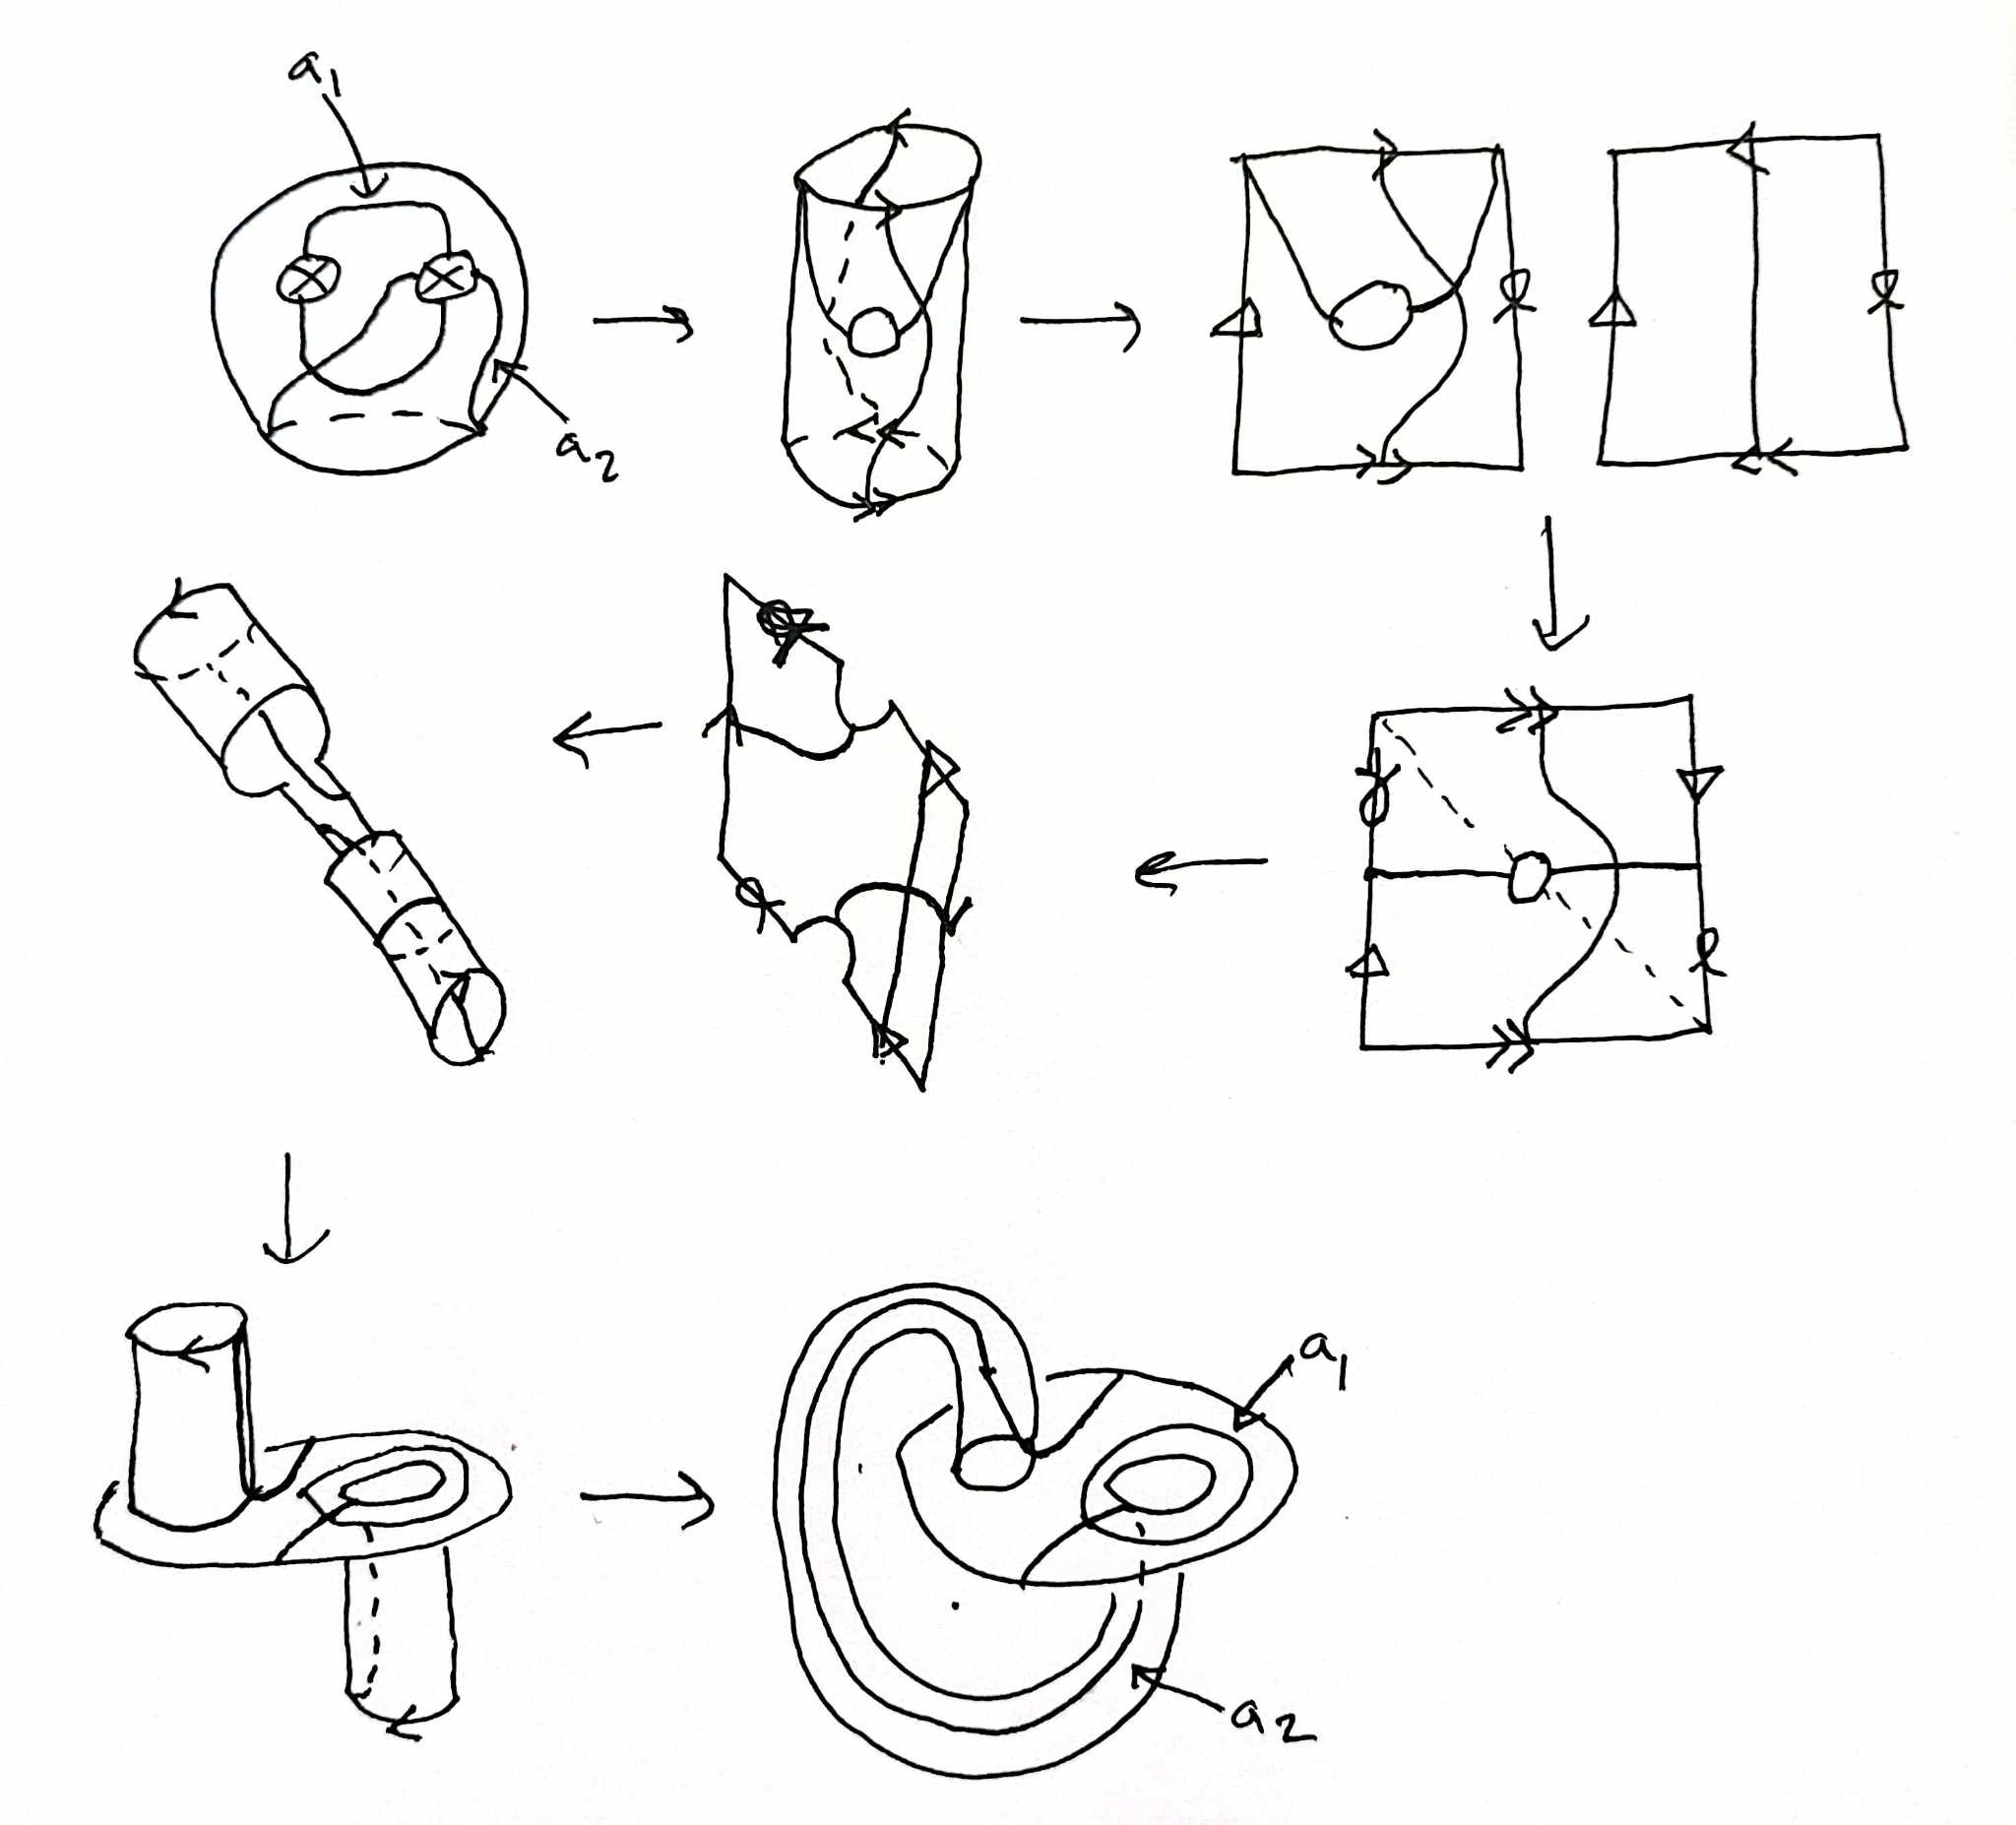
\includegraphics[width=0.7\linewidth]{part1-deformation-curve.jpg}
        \label{fig:enter-label}
    \end{figure}
\end{frame}

\begin{frame}{Proof}
    \begin{figure}
        \centering
        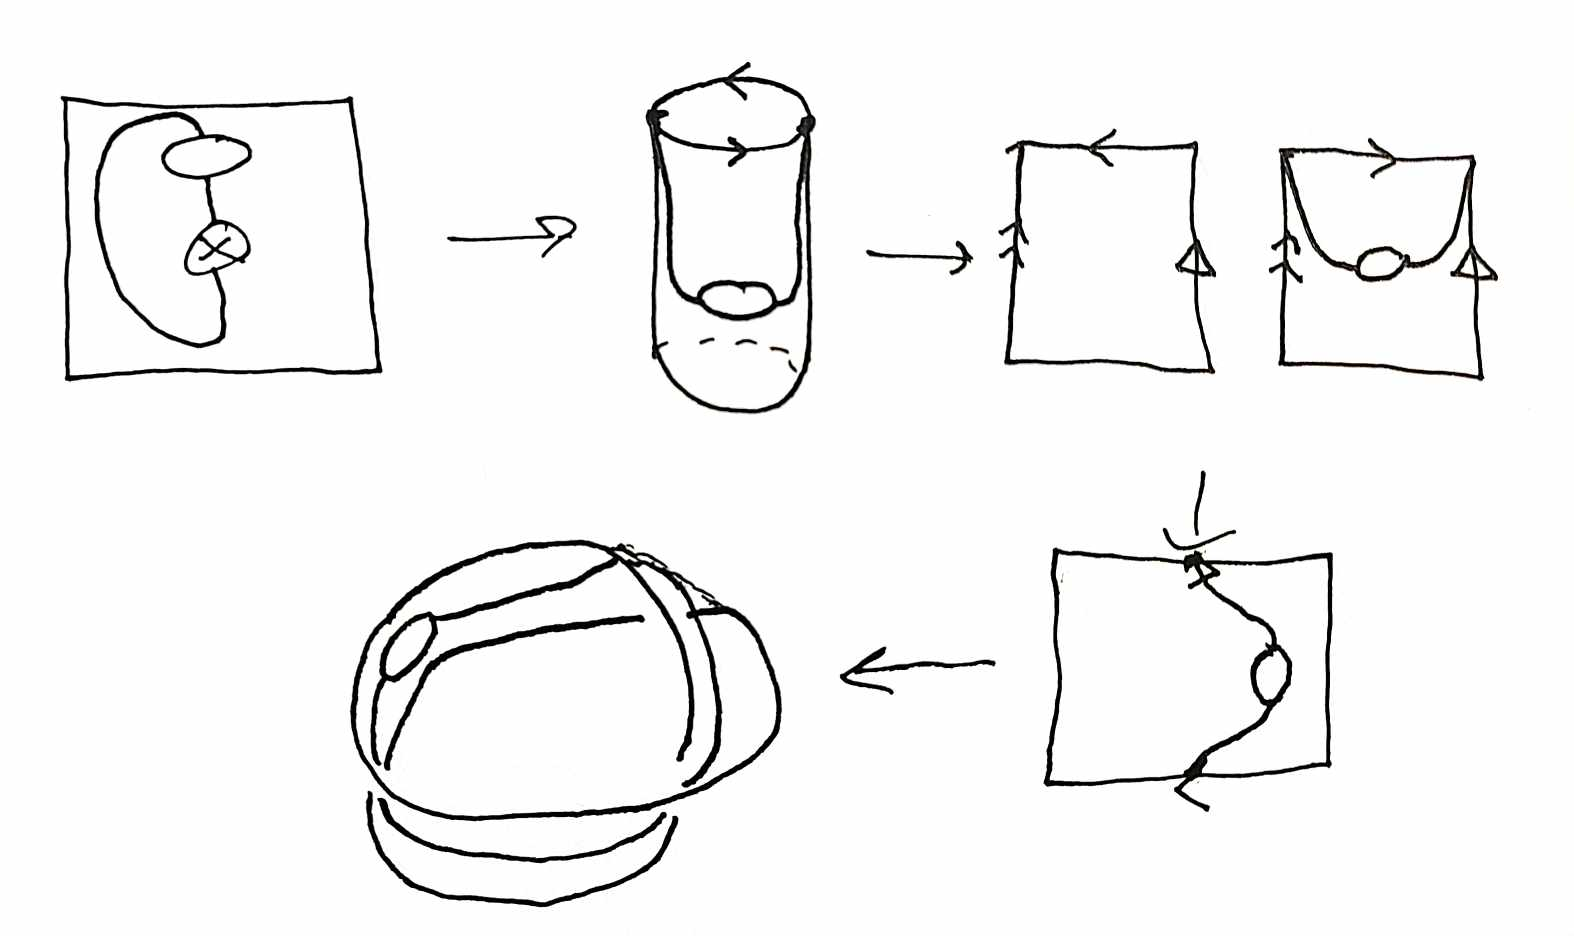
\includegraphics[width=0.8\linewidth]{part2-deformation-curve.jpg}
        \label{fig:enter-label}
    \end{figure}
\end{frame}

\begin{frame}{Proof}
    \begin{figure}
        \centering
        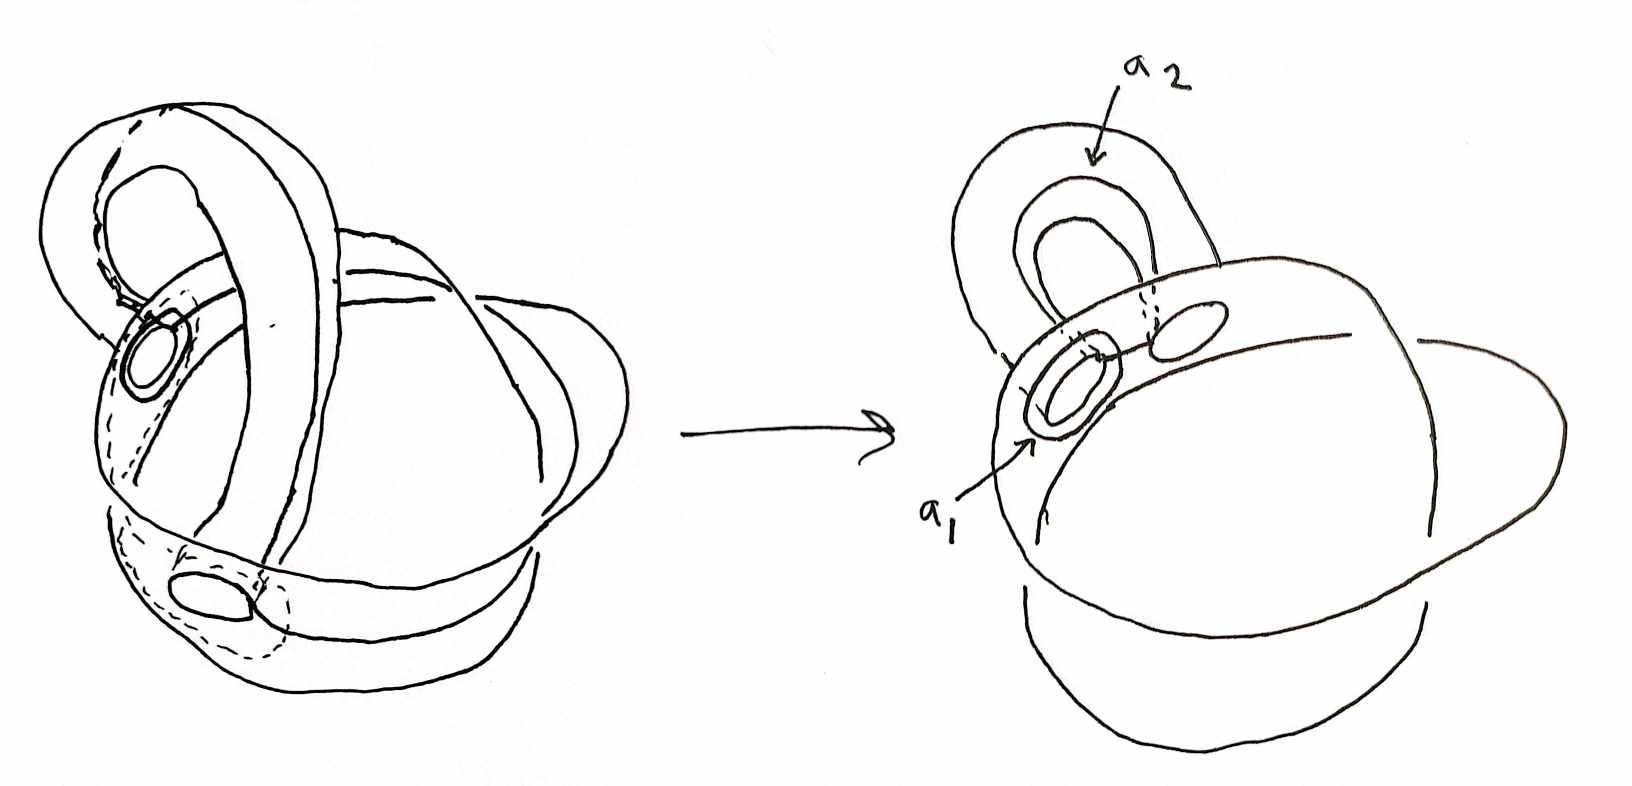
\includegraphics[width=0.8\linewidth]{klein-to-torus-curve.jpg}
        \label{fig:enter-label}
    \end{figure}
\end{frame}

\begin{frame}{Proof}
    \begin{figure}
        \centering
        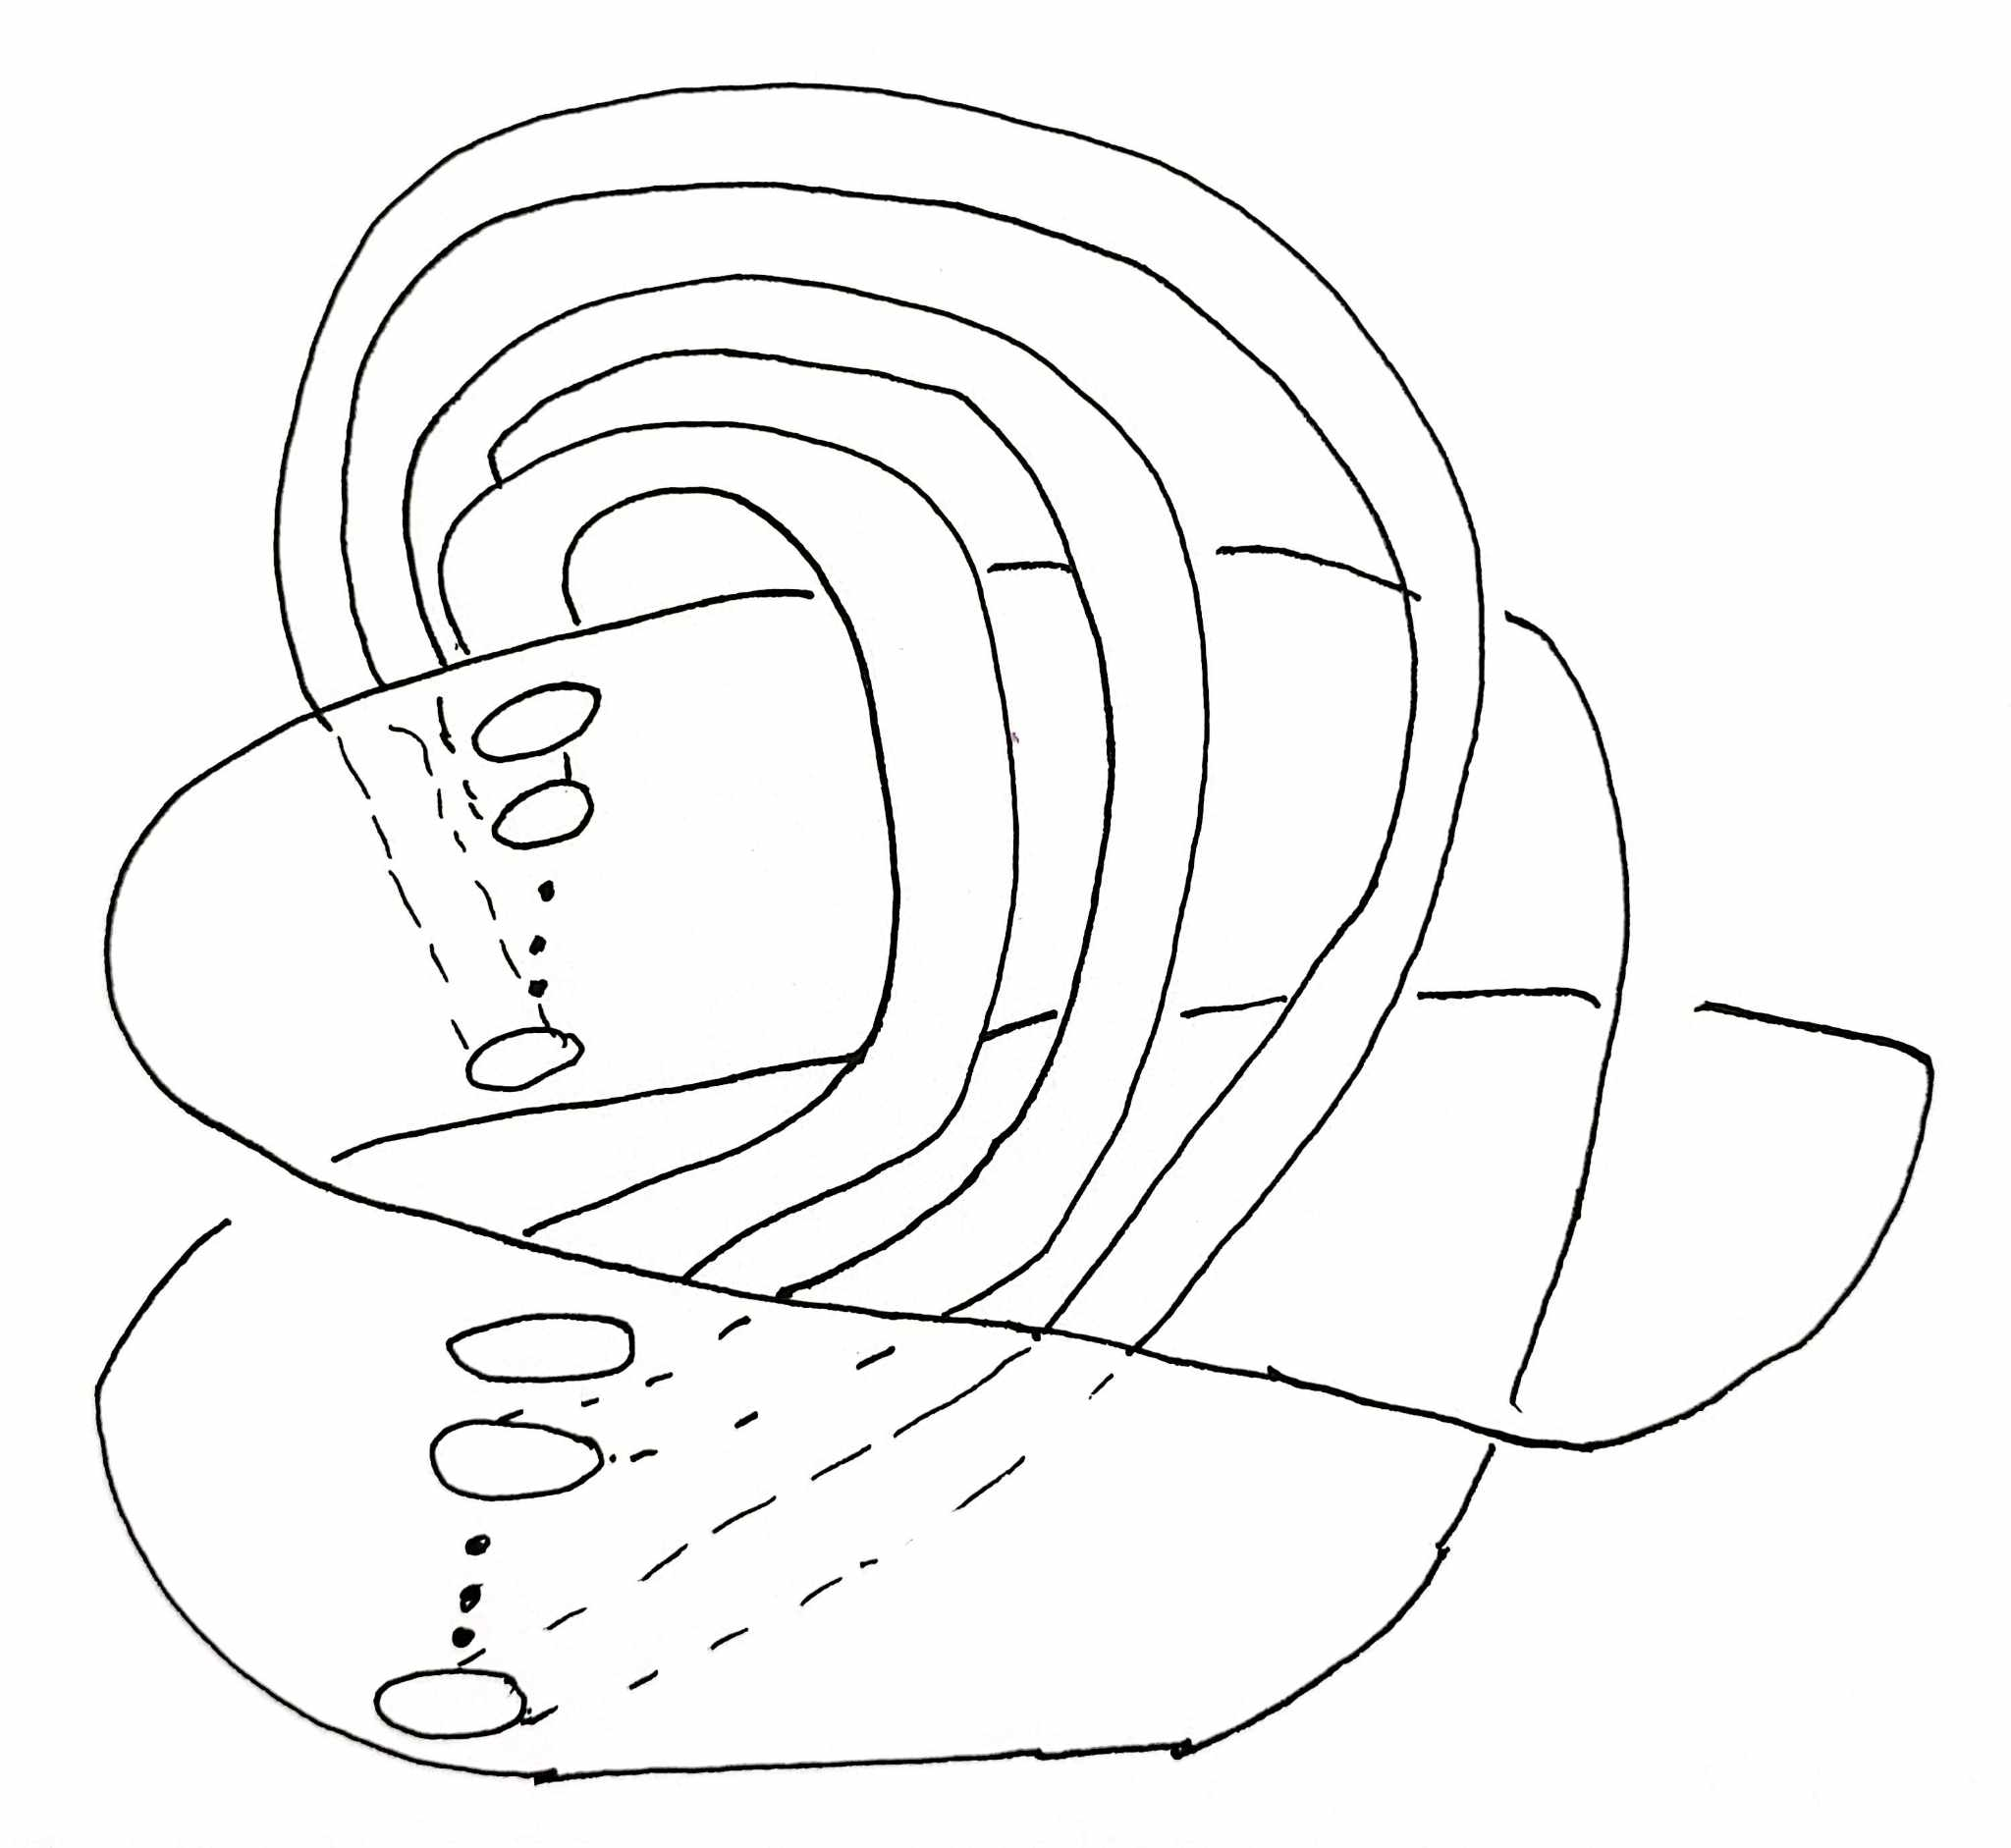
\includegraphics[width=0.5\linewidth]{many-klein-torus-curve.jpg}
        \label{fig:enter-label}
    \end{figure}
    \qed
\end{frame}



\end{document}